\documentclass[11pt]{article}
\usepackage{hyperref}
\usepackage{amsthm}
\usepackage{amsmath}
\usepackage{amsfonts}
\usepackage{tikz}
\usepackage{ wasysym }
\usepackage{fancyvrb}



\newtheorem{example}{Example}


\author{}
\title{}

\begin{document}
\pagenumbering{roman}
%\maketitle
{\Large
%Change Document name to: Graded Homework 1\_Jacob\_Nicholas
\noindent NAME:  Nicholas Jacob\\ 
EMAIL: \href{mailto: nicholascjacobphd@gmail.com}{nicholas.c.jacob-1@ou.edu}\\
STUDENT ID: \# 113578513\\
Final Project\\
COURSE: CS/DSA 4513 DATABASE MANAGEMENT\\ 
SECTION: ONLINE\\SEMESTER: FALL 2023\\
INSTRUCTOR:  DR. LE GRUENWALD\\
 SCORE:}

\newpage
\tableofcontents
\newpage
\pagenumbering{arabic}
\setcounter{page}{1}

\section{ER Diagram}
Here is my ER diagram

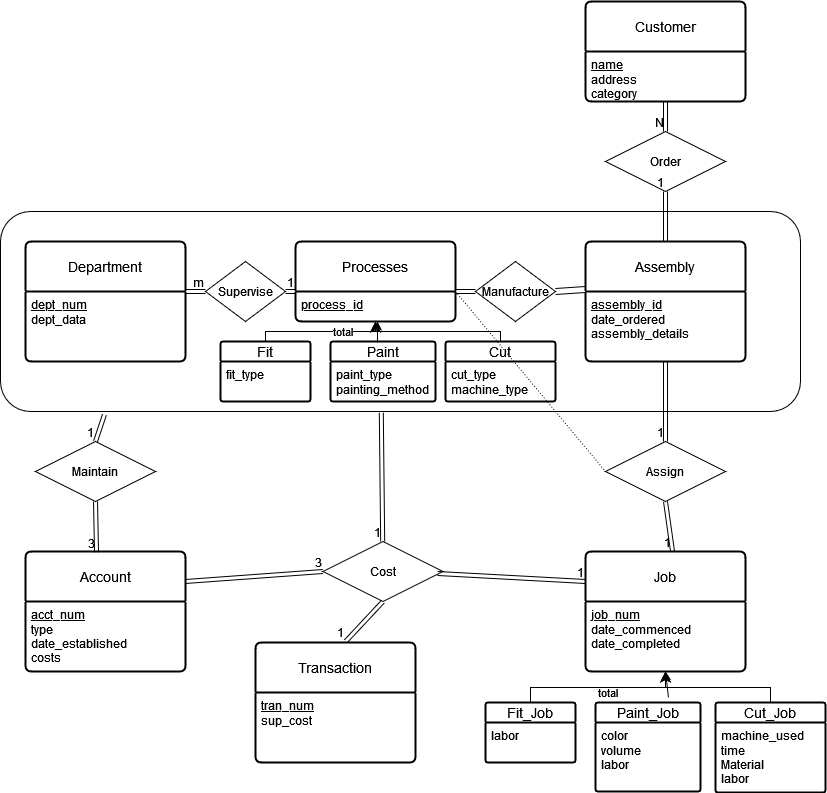
\includegraphics[width=\textwidth]{Project.png}
\newpage

\section{Relational Database Schema}

\indent Here are my schema:

Process(\underline{process\_id},process\_data)

Assemblies(\underline{assembly\_id},date\_ordered, assembly\_details)

Manufacture(\underline{process\_id},\underline{assembly\_id})

Customer(\underline{name},address, category)

Order(\underline{name},\underline{assembly\_id})

Department(\underline{dept\_num},dept\_data)

Supervise(\underline{dept\_num},\underline{process\_id})

Fit(\underline{process\_id}, fit\_type)

Paint(\underline{process\_id}, paint\_type, painting\_method)

Cut(\underline{process\_id},cutting\_type, machine\_type)

%Maintain(\underline{acct\_id}, \underline{dept\_num}, \underline{process\_id}, \underline{assembly\_id})%I think this should be cut entirely

Account(\underline{acct\_id}, type, type\_id, date\_established, costs)

Job(\underline{job\_num}, job\_date\_commenced, job\_completed)

Assign(\underline{job\_num}, \underline{assembly\_id},\underline{process\_id})

Transaction(\underline{tran\_num}, sup\_cost)

Costs(\underline{job\_num}, \underline{acct\_id},\underline{process\_id}, \underline{assembly\_id}, \underline{tran\_num},\underline{dept\_num})

Fit\_Job( \underline{job\_num}, labor)

Paint\_Job( \underline{job\_num},color,volume, labor)

Cut\_Job( \underline{job\_num}, machine\_type, time, material, labor)

\newpage
\section{Storage}
\subsection{Storage Structures}
\begin{tabular}{|p{.75in}|p{.75in}|p{.75in}|p{.65in}|p{.75in}|p{1.75in}|}\hline
Table Name & Query Number and Type & Search Key& Query Frequency& Selected File Organization & Justification\\ \hline\hline
Customer & 1 Insertion & name & 30/Day & heap on name & At the moment adding lots of data and not accessing it directly often\\ \hline 
Department & 2 Insertion& dept\_num & infrequent & Sequential on dept\_num & Since this data is added infrequently but referenced by other tables often, sequential insertion seems appropriate.\\ \hline
Process (and sub categories)& 3 Insertion & process\_id,  (sub category info) & infrequent & Sequential on process\_id (and sub category id)&  Infrequent insertion but often called\\ \hline
Supervises & 3 Insertion & process\_id and dept\_num & infrequent & Sequential on process\_id &Infrequent insertion but called often on process\_id\\\hline
Orders & 4 Insertion & name, assembly\_id& 40/Day&dynamic hash on name and ass\_id& This is a lot of orders to create each day.  These will need to be joined with other tables frequently as is happening in our insertion so it is important to be easily accessible  \\ \hline
Manufacture  & 4 Insertion & assembly\_id &40/Day (but each assembly may have many processes) &dynamic hash on assembly\_id & Frequent insertion with joins on other tables            \\ \hline
Account & 5 Insertion & type\_acct and num & 10/Day & Multitable clustering with type\_acct for clustering and num sequential& This structure will make for fast access later and there is a fair amount of additions here.\\ \hline
\end{tabular}
\newpage
\begin{tabular}{|p{.75in}|p{.75in}|p{.75in}|p{.65in}|p{.75in}|p{1.75in}|}\hline
Table Name & Query Number and Type & Search Key& Query Frequency& Selected File Organization & Justification\\ \hline\hline
Job & 6 Insertion & job\_num   &50/day& B tree on job\_num& B tree is appropriate for often inserted and often called index.     \\ \hline

Job & 7 Random Search (Insertion of job\_date\_end) & job\_num & 50/Day & $B$ tree on job\_num  &To enter completion data, you'll need a random search on job\_num.  $B$ tree will be an efficient storage for all these records \\ \hline

Transaction and Costs & 8 Random Search & tran\_no  for Transaction and tran\_num, process\_id for Costs &50/day& B tree on the tran\_no and process\_id & We'll need to update a lot of accounts here so it will be important to get to them quickly\\ \hline

Account & 9 Random Search & type = Assembly and num &200/day& B tree on num & We have previously done clustering on these attributes so this will require nothing additional to the file\\ \hline

Job  & 10 Range Search & job\_date\_commenced and job\_date\_completed & 20/day & Sequential index on both dates & Frequent call.  If put in order can retrieve data faster\\\hline

Manufacture & 11 Random Search & assembly\_id &100/day& Sequential index on assembly\_id & This index was already created for Query 4.\\\hline

Customer & 12 Range Search & name (in order) by category &100/Day & Multitable Clustering with category for clustering and name stored in a $B^+$ tree& Since this data is accessed often this table should be pre-built.  New customers are added often so $B^+$ tree storage on name will be most efficient within this multitable\\\hline

Cut\_Job & 13 Range Search & job\_num & 1/Month & Sequential Index on job\_num & Since we are doing a range search, we would like these to be in order. \\ \hline

Paint\_Job & 14 Random Search & job\_num &1/Week & Dynamic Hash function on job\_num & since we are accessing occasionally but adding lots of jobs, it would be nice to have quick access via a hash. \\ \hline
\end{tabular}
\subsection{Storage Structures on Azure}
Info on Azure indexing can be found \href{https://learn.microsoft.com/en-us/sql/relational-databases/indexes/indexes?view=sql-server-ver16}{here}.  Implementing these was a challenge.  Azure uses B trees by default on the primary keys.  This is great for random search but not so great for range searches.  Since we knew this there were a few indexes that were unnecessary to create.  Most of the rest were created especially if there were two attributes that were being indexed together.  Sequential indexes (for range sort) were done by adding the ASC or DES tag to the attribute in question.  Each index was created and added to the SQL code creating the tables necessary for indexing.

\section{SQL and Azure}

I have included my entire SQL file here.

\VerbatimInput{FinalProject.sql}

I will also include some screenshots of me utilizing SQL in Azure.  The enumeration follows the execution of each of the queries in the assignment.  I have used the naming convention in the Transact SQL as `query\#'. 

\begin{enumerate}
\item 
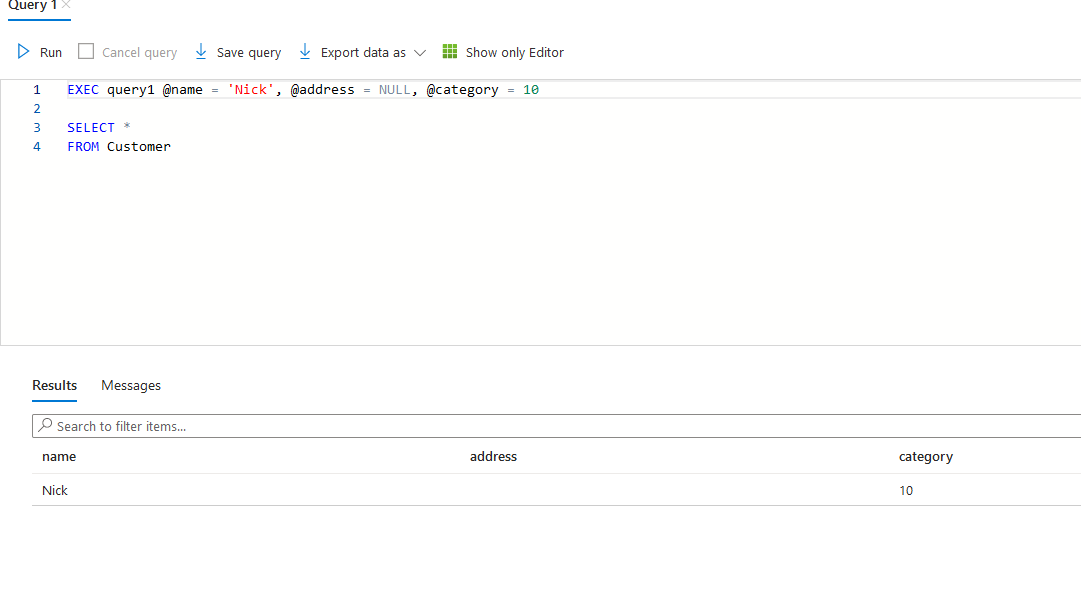
\includegraphics[width = \textwidth]{insertCust1.png}

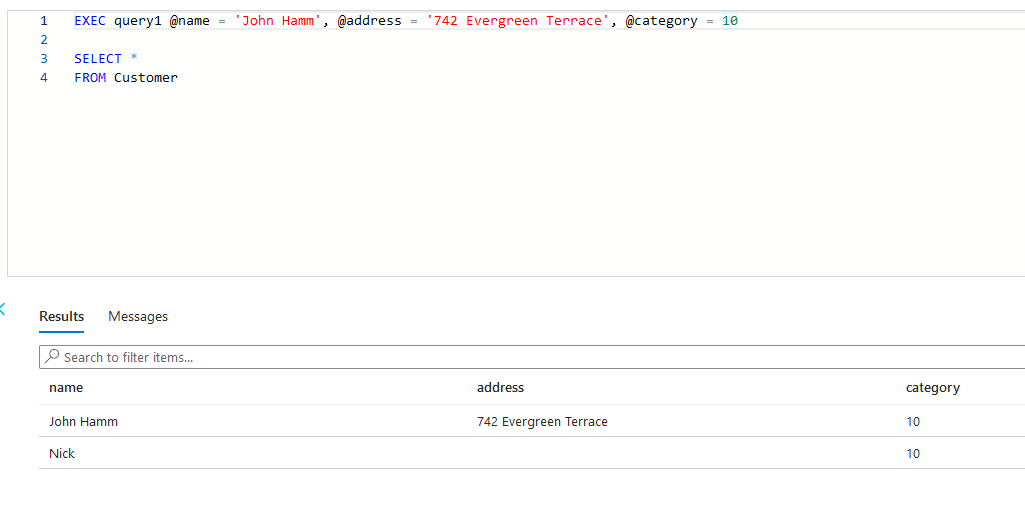
\includegraphics[width = \textwidth]{insertCust2.png}

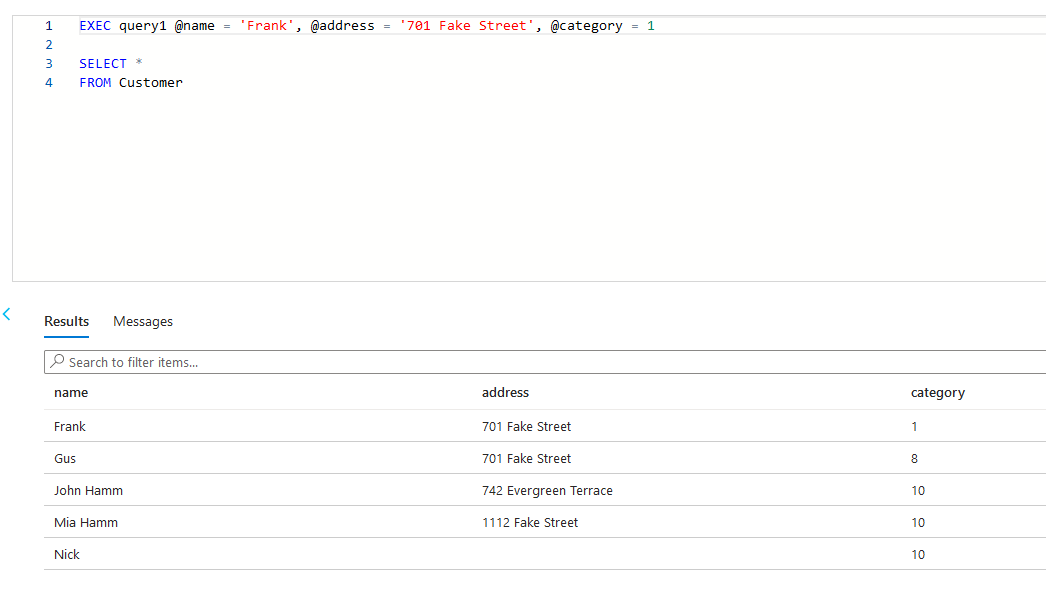
\includegraphics[width = \textwidth]{insertCust3.png}

\item
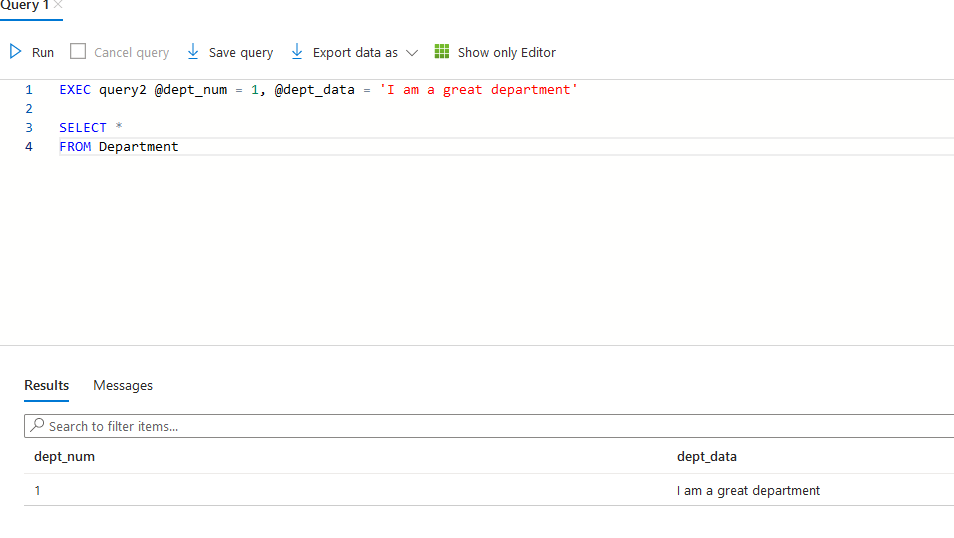
\includegraphics[width = \textwidth]{insertDept1.png}

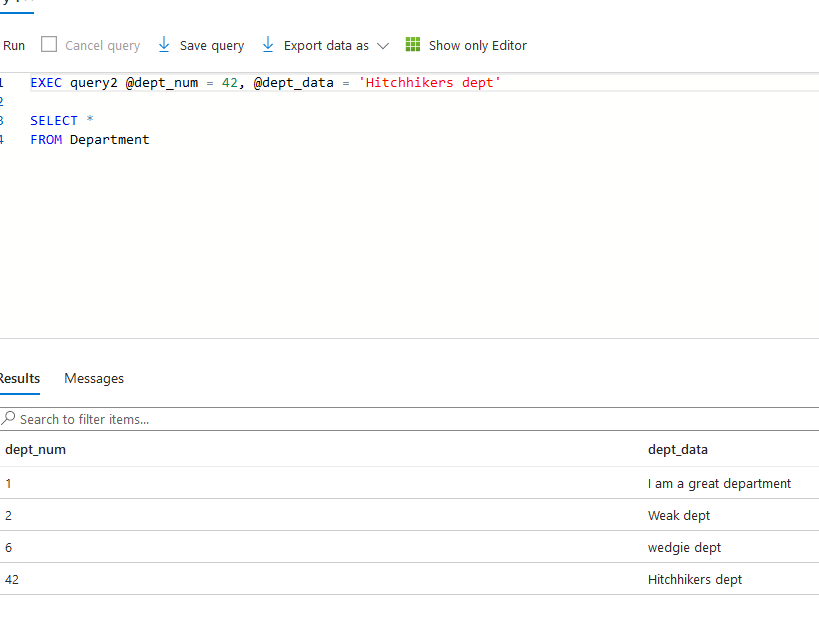
\includegraphics[width = \textwidth]{insertDept2.png}

\item
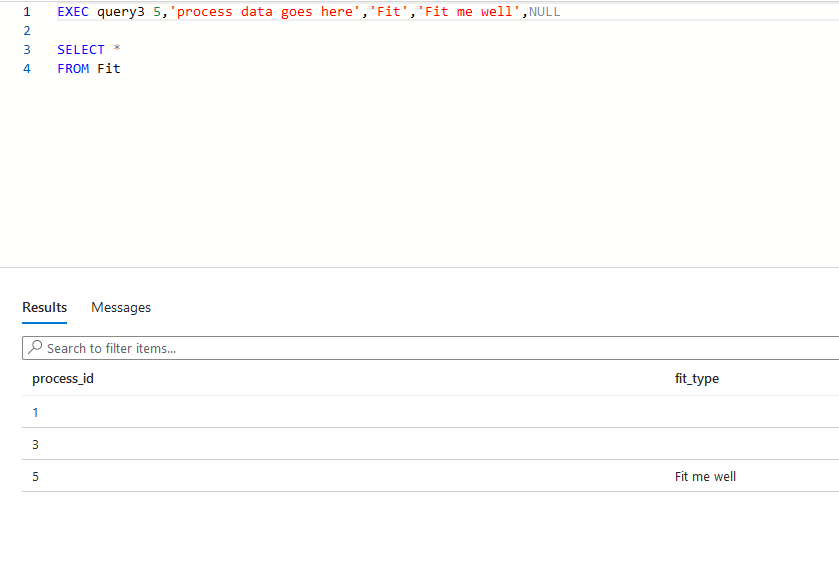
\includegraphics[width = \textwidth]{insertProcess1.png}

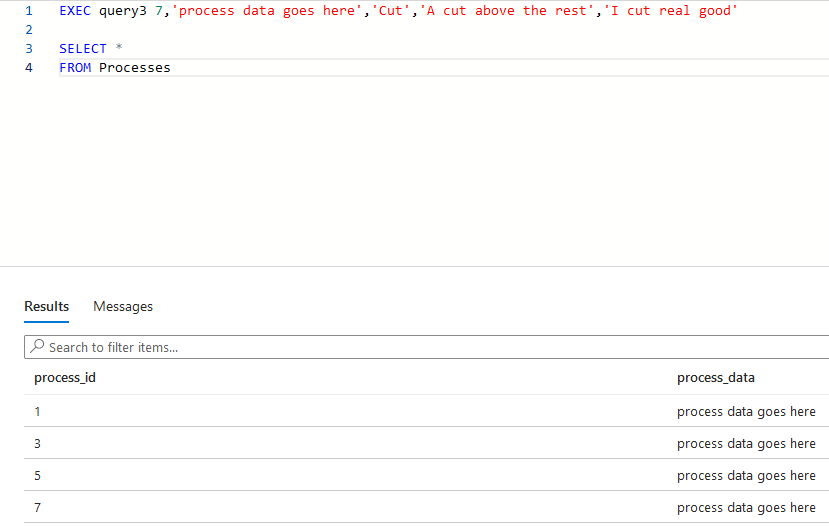
\includegraphics[width = \textwidth]{insertProcess2.png}

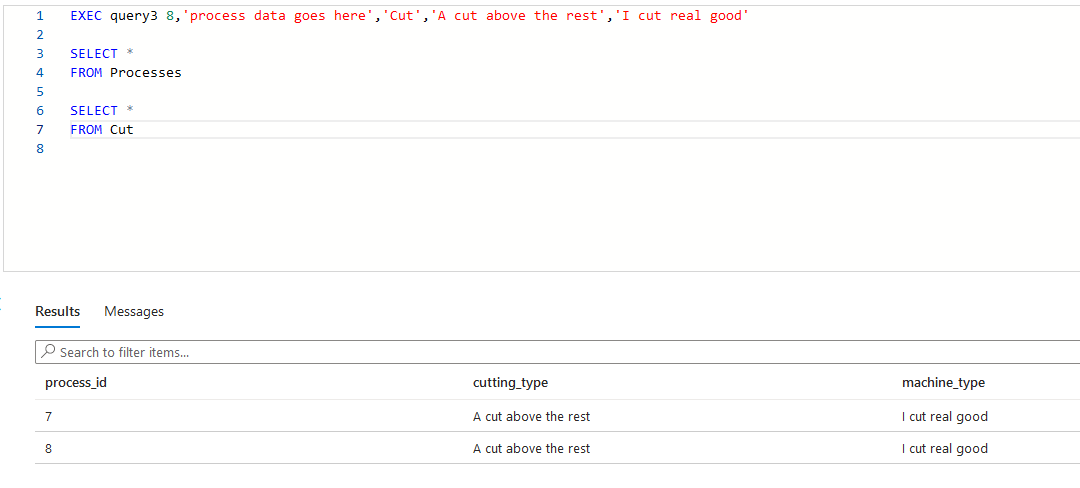
\includegraphics[width = \textwidth]{insertProcess3.png}

\item
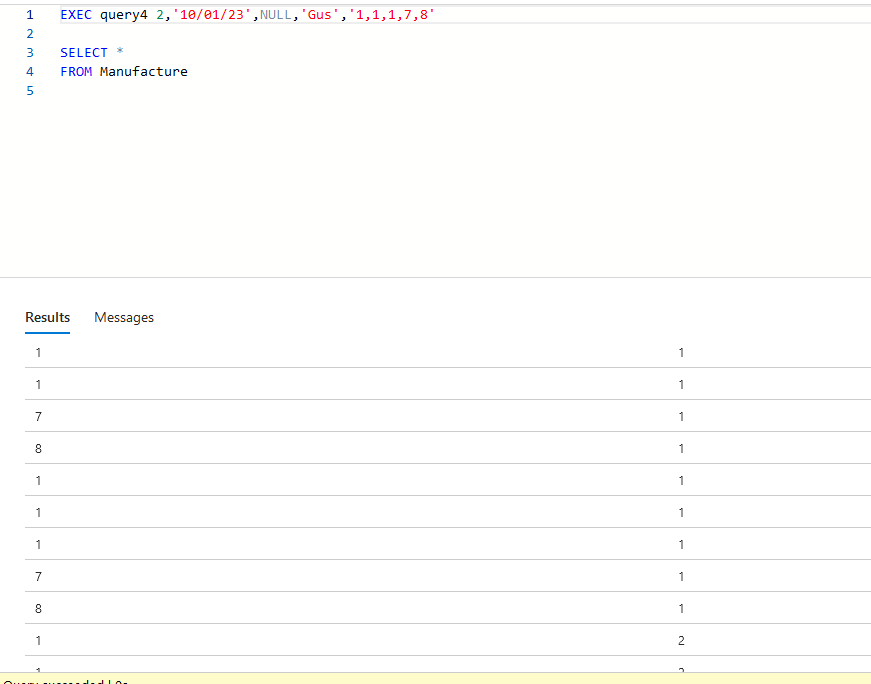
\includegraphics[width = \textwidth]{insertAssembly1.png}

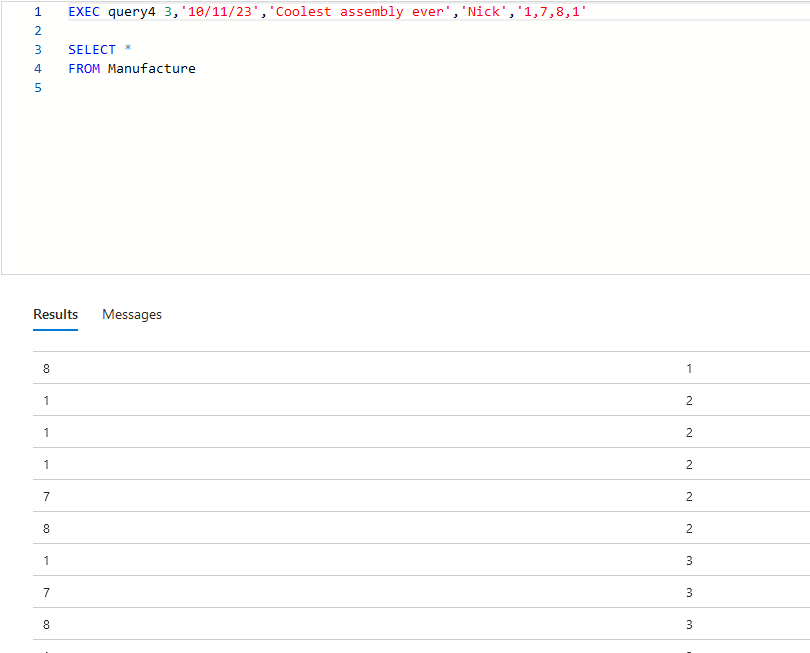
\includegraphics[width = \textwidth]{insertAssembly2.png}

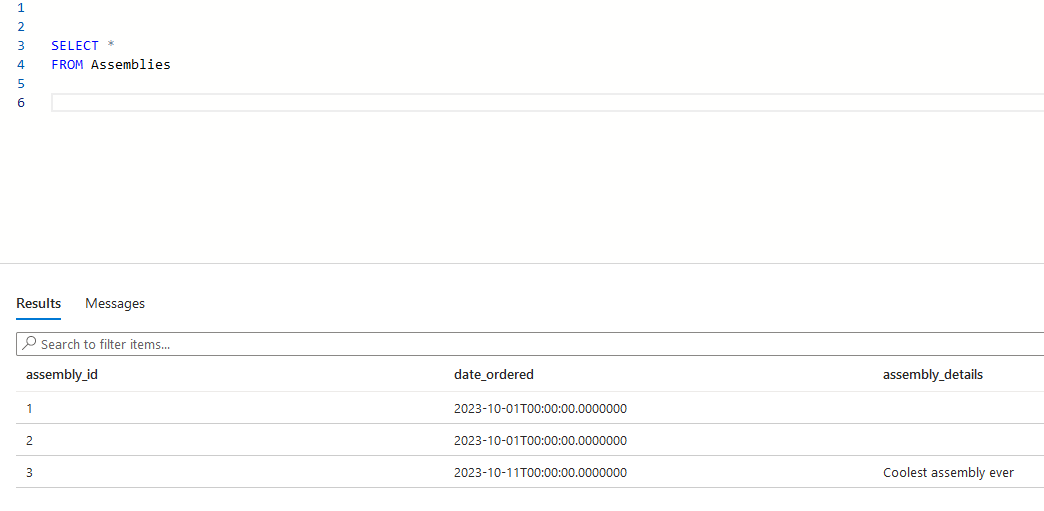
\includegraphics[width = \textwidth]{insertAssembly3.png}

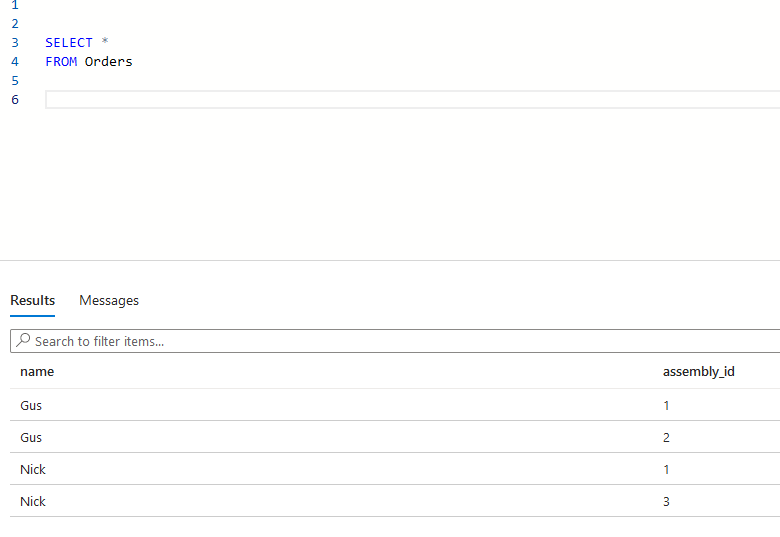
\includegraphics[width = \textwidth]{insertAssembly4.png}

\item %#5
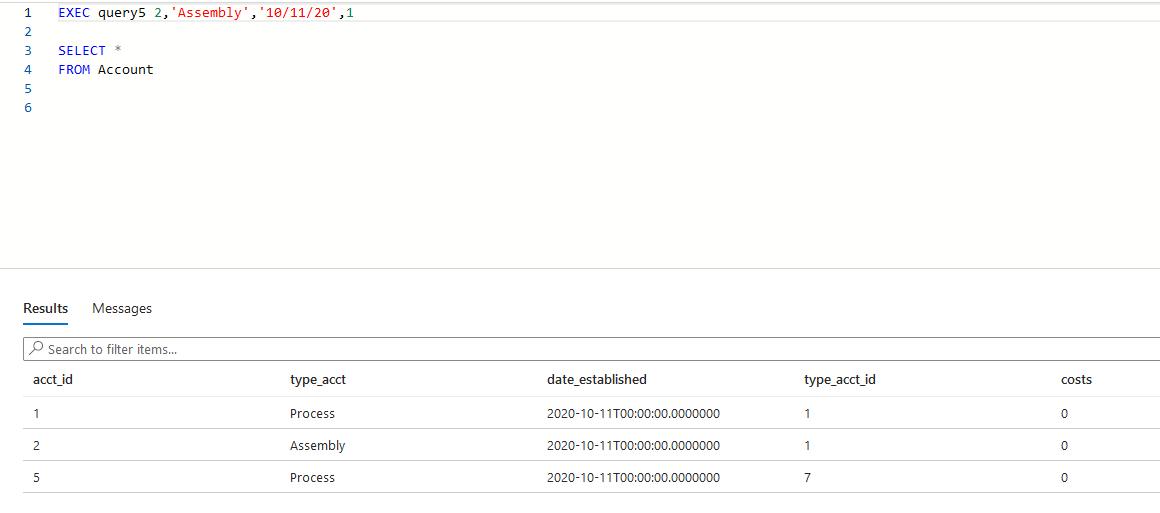
\includegraphics[width = \textwidth]{insertAcct1.png}

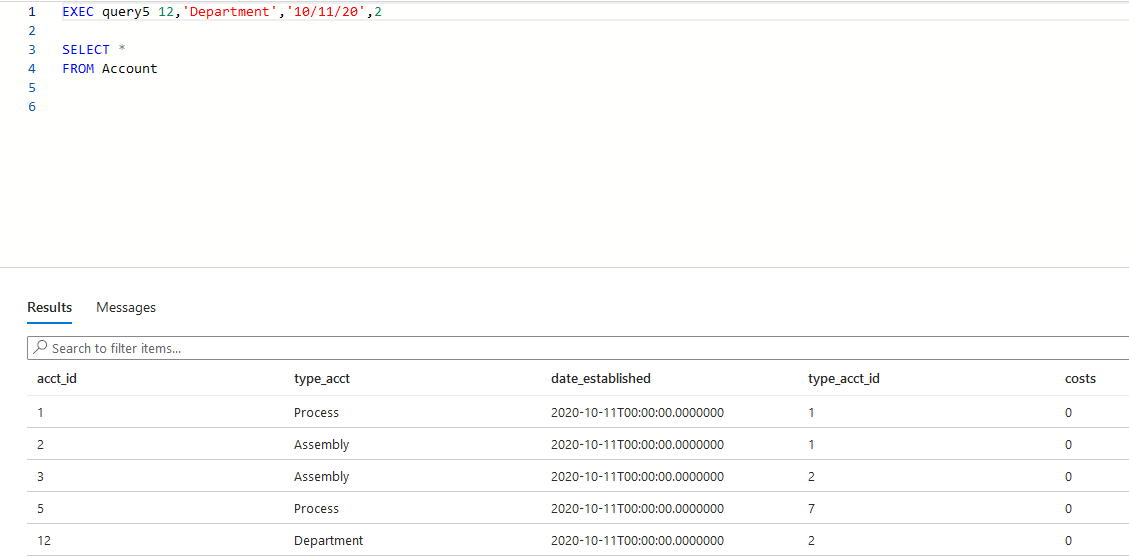
\includegraphics[width = \textwidth]{insertAcct2.png}
\end{enumerate}
\section{SQL and Java}
\subsection{SQL Transact}
I put the transact calls in the same file that created the tables.  If I have time, I should split this up...
\VerbatimInput{FinalProject.sql}

\subsection{Java Implementation}
\VerbatimInput{FinalProject.java}
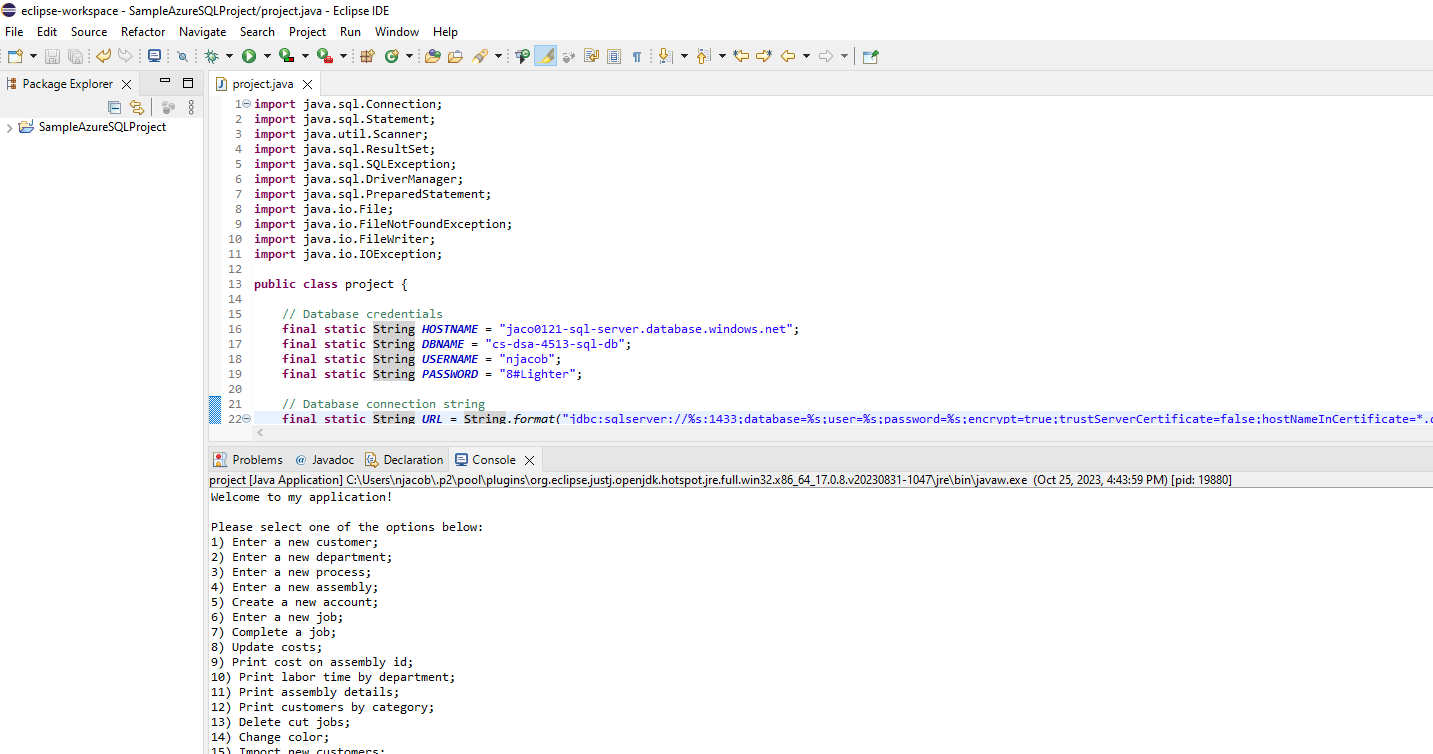
\includegraphics[width = \textwidth]{JavaSuccess.png}
\section{Java Execution}
\section{Web Database}
\subsection{Source Code}
{\bf Data Handler}
\VerbatimInput{DataHandler.java}

\noindent { \bf Add customer}
\VerbatimInput{add_customer.jsp}

\noindent {\bf Add customer form}
\VerbatimInput{add_customer_form.jsp}

\noindent {\bf Get all customers}
\VerbatimInput{get_all_customers.jsp}

\noindent {\bf Get all customers form}
\VerbatimInput{get_all_customers_form.jsp}
\subsection{Screenshots}
Holy cow I didn't think I would get this to work!

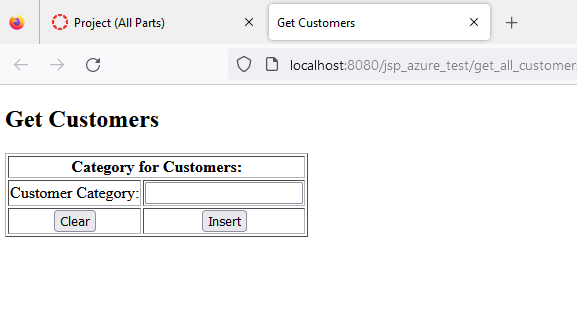
\includegraphics[width = \textwidth]{web1.png}

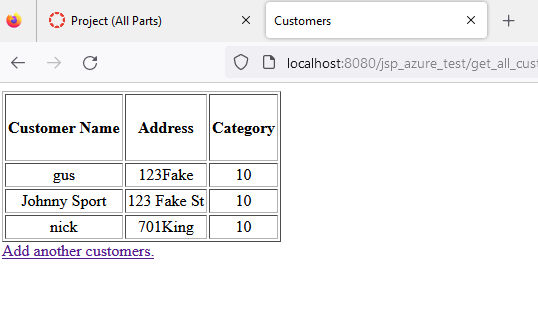
\includegraphics[width = \textwidth]{web2.png}

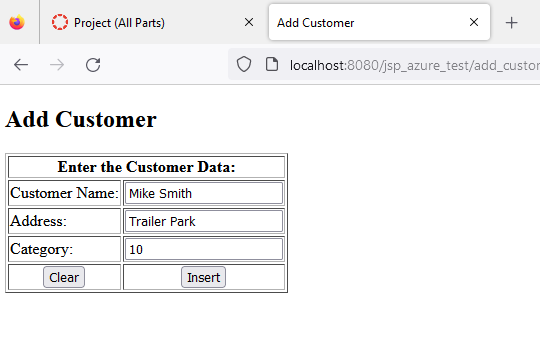
\includegraphics[width = \textwidth]{web3.png}

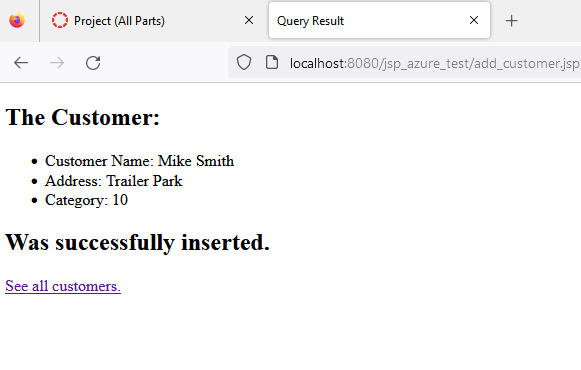
\includegraphics[width = \textwidth]{web4.png}

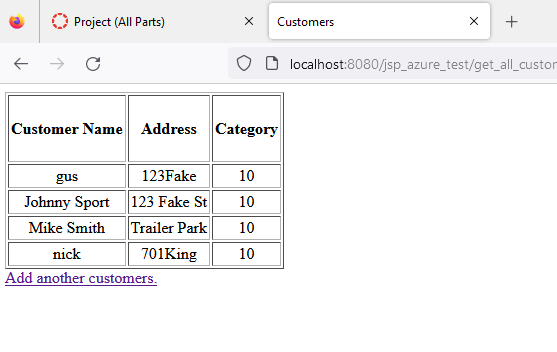
\includegraphics[width = \textwidth]{web5.png}
\end{document}